%!TEX TS-program = ../make.zsh

\section{Theoretical Concepts}
\label{sec:theoretical_background}

\subsection{Neutrinos}
\label{sec:neutrinos}

Neutrinos are particles that primarily interact with other particles through the \textit{weak interaction} and have very small probabilities of interacting with other particles, allowing them to cross matter almost unhindered. While this makes them interesting messenger particles for observing far-distant astronomical sources and phenomena, because they are long ranging and arrive undeflected and unscattered, it also makes their detection challenging due to the large amount of detector medium required. \cite{lexikonderphysik, instrumentation}

Within the \textit{standard model of particle physics} (see figure \ref{fig:Pheith9i}), the electron neutrino, $\Pnue$, the muon neutrino, $\Pnum$, and the tau neutrino $\Pnut$, are \textit{leptons} without electrical charge and couple to the $\PWpm$ and $\PZz$ bosons.

\begin{figure}[htbp]
  \smallerimage{standard-model}
  \caption{Particles of the standard model of particle physics. Together with the electron, the muon, and the tau, the neutrinos form the group of leptons, which do not participate in \textit{strong interactions}. As neutrinos also do not participate in the \textit{electromagnetic interaction}, their primary interaction channel is through \textit{weak interactions}. Image based on: \cite{standardmodel}}
  \label{fig:Pheith9i}
\end{figure}

As the \textit{mass eigenstates} $\Pnu_i$ of neutrinos that describe neutrinos in the context of their propagation through spacetime, are not identical to the neutrino \textit{flavor eigenstates} $\Pnulepton$ that describe neutrinos participating in weak interactions, neutrinos are subject to quantum mechanical phenomena as \textit{neutrino oscillations}. \cite{particledatareview}

$$
  \ket{\Pnulepton} = \sum_{i=1}^N U_{\Plepton i}\,\ket{\Pnu_i}, \ \ \ \Plepton \in \{ \Pe, \Pmu, \Ptau \}
$$

Determining the mixing matrix $U_{\Plepton i}$ that connects the mass eigenstates to the flavor eigenstates, is part of \icecube's scientific objectives.

Neutrinos generated by interactions of cosmic-ray particles in the Earth's atmosphere, \textit{atmospherical neutrinos}, have energies in the GeV to TeV scale. \textit{Astrophysical neutrinos}, generated by high-energy phenomena in the universe, have energies up to the PeV scale. \cite{instrumentation}


\subsection{Neutrino Interactions Relevant to \icecube}
\label{sec:neutrino_interactions}

The primary interaction channel for detecting neutrinos in \icecube is deep-inelastic scattering of neutrinos with quarks of nuclei in the detector material or nearby rock (see figure \ref{fig:Phei1oob}). \cite{energyreco}

\begin{figure}[htbp]
  \centering
  \subcaptionbox{Neutral-current neutrino interaction through $\PZz$ bosons.}{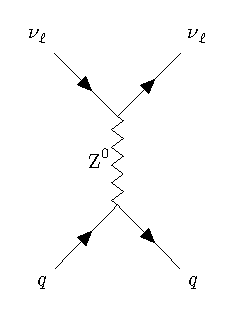
\includegraphics[width=0.3\textwidth]{img/feynman-neutral}\vspace*{2mm}}\hspace{1cm}
  \subcaptionbox{Charged-current neutrino interactions through $\PWpm$ bosons.}{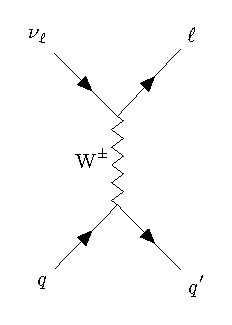
\includegraphics[width=0.3\textwidth]{img/feynman-charged}}
  \caption{Feynman diagrams showing neutrinos $\Pnulepton$ interacting with quarks $\Pquark$ of nuclei of the ice or nearby rock through $\PZz$ and $\PWpm$ bosons, producing leptons $\Plepton$---that is to say electrons $\Pe$, muons $\Pmu$, tau particles $\Ptau$---and quarks. Time evolves to the right in these diagrams.}
  \label{fig:Phei1oob}
\end{figure}

These interactions lead to three different kind of event signatures in the \icecube detector.

\paragraph{Shower- or Cascade-Like Events}
In both, interactions through $\PZz$ bosons (\textit{neutral-current interactions}) and through $\PWpm$ bosons (\textit{charged-current interactions}), hadronic showers, that is to say cascades of secondary particles, are created as energy is transferred from the incoming neutrino to the outgoing quark. If the outgoing lepton is an electron, this may also create an accompanying electromagnetic shower. \cite{energyreco}

\begin{align*}
  & \text{neutral current:} & \Pnulepton + \text{nucleon} & \rightarrow \Pnulepton + \text{hadron} \ \ \ \ \ \ \Plepton \in \{ \Pe, \Pmu, \Ptau \}                             & \\
  &                         &                             & \rightarrow \Pnulepton \text{ (escapes) } + \text{hadronic shower}  & \\ \\
  & \text{charged current:} & \Pnue + \text{nucleon}      & \rightarrow \Pe + \text{hadron}                                     & \\
  &                         &                             & \rightarrow \text{electromagnetic shower} + \text{hadronic shower}  & \\
\end{align*}

\paragraph{Track-Like Events}
If the outgoing lepton is a muon, this creates track-like event signatures as muons travel long distances. TeV muons may travel several kilometers in the antarctic ice, while light is emitted along the track. \cite{skysearch, mmc}

\begin{align*}
  & \text{charged current:} & \Pnum + \text{nucleon}      & \rightarrow \Pmu + \text{hadron}                                    & \\
  &                         &                             & \rightarrow \text{muon track} + \text{hadronic shower}              & \\
\end{align*}

\paragraph{Double-Bang Events}
If the outgoing lepton is a tau, the tau will create a track, but the track will only be a couple of meters long, before the tau, which has sufficient mass, decays into another hadronic shower, creating a so-called \textit{double-bang signature}, that is to say two hadronic showers joined by a short track. \cite{skysearch, energyreco, particledatareview}

\begin{align*}
  & \text{charged current:} & \Pnut + \text{nucleon}      & \rightarrow \Ptau + \text{hadron}                                   & \\
  &                         &                             & \rightarrow \text{tau track} + \text{hadronic shower}               & \\
  &                         &                             & \rightarrow \text{hadronic shower} + \text{hadronic shower}         & \\
\end{align*}

The event signatures, how they appear in the \icecube detector, are visualized in figure \ref{fig:eeQuaef6}.

\begin{figure}[htbp]
  \centering
  \subcaptionbox{Cascade-like event: The cascade is completely contained within the detector and deposits a total of $1141\TeV$ energy within the detector. Image and data source: \cite{evidence2013,energyreco}}{\halfimage{evidence2013-event-20}}\hfill
  \subcaptionbox{Track-like event: The muon track starts within the detector and deposits a total of $71\TeV$ of energy within the detector before it leaves the detector volume. Image and data source: \cite{evidence2013,energyreco}}{\halfimage{evidence2013-event-5}}\hfill
  \subcaptionbox{Simulated double-bang event: The earlier (red) cascade has been created from the primary neutrino interaction vertex. The tau travels from the position of the first cascade for a short distance, creating a track, before decaying into another later (green) cascade. Image source: \cite{nufact2018}}{\halfimage{nufact2018-double-bang}}\hfill
  \caption{Visualization of examples for the different event signatures of neutrino events observed with \icecube. The spheres represent the energy registered by the respective detector module. The color indexes the time information: Red is the beginning of the event, green the middle, and blue the end of the event.}
  \label{fig:eeQuaef6}
\end{figure}


\subsection{Cherenkov-Light Emission}
\label{sec:cherenkov}

When charged particles, both the primary lepton and particles within the cascades, move through the detector medium faster than the phase velocity of light within this medium, they emit so-called \textit{Cherenkov radiation}, which are photons with wavelengths in the visible and the near ultra violet spectrum. \cite{energyreco, instrumentation, skysearch}

The light emission is not isotropic: Photons are emitted under an angle $\phi$ relative to the direction of propagation of the charged particle. \cite{physiklexikon}

$$
  \cos \phi = \frac{1}{\beta\,n} = \frac{c'}{v}, \ \ \ \beta = \frac{v}{c}, \ \ \ c' = \frac{c}{n}
$$

$n$ is the refractive index of the medium, $c'$ the speed of light within the medium, $c$ the speed of light in vacuum.

The virtual photon field of the charged particle moving through the medium polarizes the atoms in the medium. Each resulting electric dipole is a source of electromagnetic radiation. But as each dipole arranges towards the charged particle, integrating over the whole spatial sphere around the charged particle, the net emitted radiation vanishes if the charged particle's velocity $v$ is smaller than the speed of light $c'$ in the medium. For higher velocities, the coulomb field of the charged particle can only polarize the atoms within a cone with an opening angle of $2\phi$, the \textit{Cherenkov cone}, resulting in a net photon emission perpendicular to the surface of the cone. \cite{physiklexikon}

Per GeV of secondary particle shower energy within the detector, an order of $10^5$ visible Cherenkov photons are created. \cite{instrumentation}

\begin{figure}[htbp]
  \centering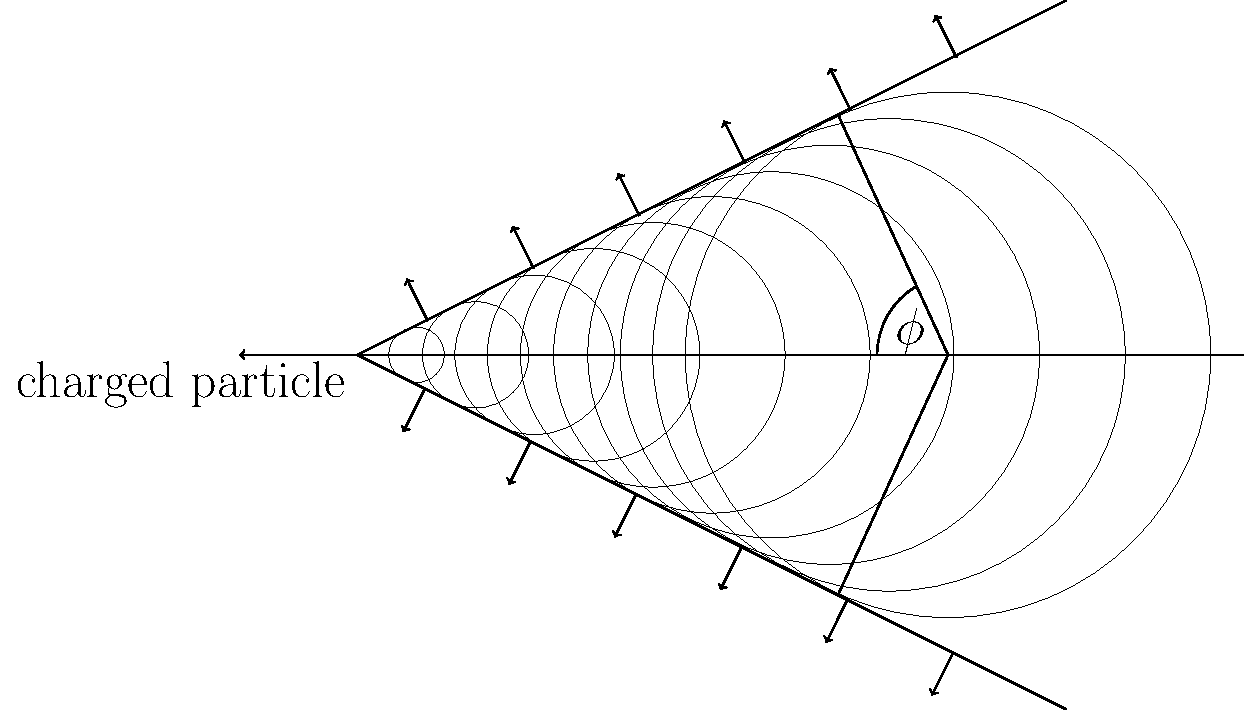
\includegraphics[width=0.3\textwidth]{img/cherenkov}
  \caption{Visualization of the \textit{Cherenkov cone}: A charged particle moves through a medium with a velocity $v>c'$ greater than the phase velocity $c'$ of light within this medium. Due to the limited speed of light being smaller than the speed of the charged particle, polarization effects are not isotropic, but \textit{Cherenkov photons} are emitted under an angle $\phi$ relative of the direction of motion of the charged particle.}
  \label{fig:ehai2Ahj}
\end{figure}


\subsection{Photon Absorption and Scattering}
\label{sec:scattering}

The propagation of light through a medium depends on the optical properties of that medium, in particular the velocity of light within that medium, the scattering probability and the absorption probability. \cite{lundberg}
% lundberg, page 4

The absorption of light for the relevant wavelength range is caused by electronic and molecular excitation processes \cite{lundberg}
% lundberg, page 4
and is quantified by the \textbf{absorption length} $\lambda\abs$, which is the mean of the exponentially distributed free path length to absorption \cite{lundberg}.
% lundberg
Therefore, in accordance with the \noun{Beer-Lambert law}, the absorption length is the path length that light needs to travel within a medium to have its intensity drop to $\sfrac{1}{\e}$ of its original intensity. \cite{lexikonderphysik}
% lexikonderphysik, Band 1, Absorptionslänge
% Absorption lengths in the South-Polar ice are in the order of $100\m$ and can in clear ice layers in the absence of dust even exceed $200\m$. \cite{ackermann}
% ackermann, page 5, paragraph 12
Absorption lengths in the South-Polar ice vary between $10\m$ in dusty regions and $280\m$ in very clear ice layers. \cite{ackermann, ppcpaper, icepaper}

The scattering of light off microscopic scattering centers, such as sub-millimeter-sized air bubbles and micron-sized dust grains \cite{Price1997, ackermann} is the dominant scattering mechanism in glacial ice \cite{Askebjer1997, lundberg}. This scattering can be modeled using the more general \noun{Mie scattering} theory, which describes the scattering of electromagnetic radiation off small, spherical masses of material with refractive indices differing from the refractive index of its surroundings. \cite{Mie1908, ackermann, lundberg}

\noun{Mie scattering} gives the distribution of the scattering angle $\theta$ for any wavelength and scattering center size. For ice, this distribution is approximated using a one-parameter \noun{Henyey-Greenstein} (HG) phase function $p_\text{HG}(\theta; \tau)$, where the one parameter $\tau$ is the mean cosine of the scattering angle. \cite{lundberg}

$$ p_\text{HG}(\theta; \tau) = \frac{1 - \tau^2}{2(1 + \tau^2 - 2\tau\, \cos \theta)^\frac{3}{2}}, \ \ \ \tau = \meancostheta $$

The South-Polar ice has shown to be preferentially forward scattering with a mean cosine of the scattering angle of $\meancostheta = 0.94$ with only a weak dependence on the wavelength. \cite{ackermann}
% ackermann, paragraph 9

The \textbf{scattering length} $\lambda\sca$, which is also called \textbf{geometric} scattering length, is the mean of the exponentially distributed free path and thereby the average distance between scatterings. \cite{ackermann}

% https://github.com/fiedl/hole-ice-study/issues/52 - Effective scattering length
A related and often used quantity is the \textbf{effective scattering length} $\lambda\esca$, which is the distance that light needs to propagate through a turbid medium before the photon directions are completely randomized. \cite{lundberg}

\begin{equation}
  \lambda\esca = \frac{\lambda\sca}{1 - \meancostheta}
\end{equation}

In a medium with isotropic scattering, the geometric and the effective scattering lengths are the same. In a preferentially forward scattering medium like the South-Polar ice, the original direction of a sample of photons is tendentially retained for several scattering steps until the photon direction of the sample is isotropized. The projection of the net velocity vector on the original direction is decreased on average by $\meancostheta$ for each scattering. \cite{lundberg}

After $n$ scatterings, the effectively transported forward distance along the original direction is $\lambda\sca\,\sum_{i=0}^n \meancostheta^i$, such that in the limit of many scatterings, $n \rightarrow \infty$, the effectively transported forward distance becomes the effective scattering length. \cite{lundberg, ackermann}

$$ \lim_{n \rightarrow \infty} \lambda\sca\,\sum_{i=0}^n \meancostheta^i = \frac{\lambda\sca}{1 - \meancostheta} = \lambda\esca $$

% Typical scattering length:
% average esca = 25m \cite{lundberg}
% scattering lengths between 5m and 90m in the detector volume \cite{ppcpaper}
% effective scattering coefficient for 400nm between 0.011/m and 0.2/m \cite{icepaper} fig. 16, corresponding to esca=5m to 90m esca

Typical effective scattering lengths within the South-Polar ice are in the order of $25\m$ \cite{lundberg} and range from $5\m$ to $90\m$ in the detector volume \cite{icepaper}, corresponding to the geometric scattering length ranging from $0.3\m$ to $5.4\m$.

% https://github.com/fiedl/hole-ice-study/issues/51 - point particles
Light interference effects are ignored during photon propagation as the average distance between the scattering centers is large compared to the photon wavelength. \cite{ackermann}

Also, despite modeling different ice regions with abrupt boundaries in the simulations of this study, the physical boundaries are assumed such that refractive index variations are continuous. Hence reflection at the medium boundaries is ignored in simulations. \cite{lundberg}
